\documentclass[11pt,a4paper]{article}
\usepackage[margin=2.4cm]{geometry}
\usepackage{amsmath,amssymb,amsthm}
\usepackage{booktabs}
\usepackage{graphicx}
\usepackage{caption}
\usepackage[round,authoryear]{natbib}
\usepackage[hidelinks,pdfauthor={Anonymous},pdftitle={What Public Debt Statistics Establish About Interest-Rate Exposure}]{hyperref}
\usepackage{enumitem}
\setlist{nosep,leftmargin=1.6em}
\captionsetup{font=small,labelfont=bf}
\newtheorem{proposition}{Proposition}
\newtheorem{lemma}[proposition]{Lemma}
\newtheorem{theorem}[proposition]{Theorem}
\newtheorem{corollary}[proposition]{Corollary}
\theoremstyle{remark}
\newtheorem{remark}[proposition]{Remark}
\newcommand{\ov}{\operatorname{ov}}
\IfFileExists{build_info.tex}{\newcommand{\buildinfo}{git unversioned}
}{\newcommand{\buildinfo}{unversioned build}}

\title{What Public Debt Statistics Establish About\\Interest-Rate Exposure\\[4pt]
\large Sharp bounds, exact certificates and the value of additional disclosure,\\ illustrated with UK and US debt data}
\author{Anonymous}
\date{13 October 2026\thanks{Version 1.1.0-candidate. DOI: \href{https://doi.org/10.5281/zenodo.23337976}{10.5281/zenodo.23337976}. Code, permitted source data, exact model snapshots, results and certificates accompany the paper; restricted source originals require separate retrieval.}}

\begin{document}
\maketitle

\begin{abstract}
\noindent
Public debt statistics constrain, but need not identify, interest-rate exposure. Under a declared refinancing model, we compute sharp bounds over all portfolios consistent with published moments, retaining exact rational optimality certificates. UK and US instrument-level demonstrations show how broad maturity buckets can leave large uncertainty. In the gross UK model, one additional within-year mean reduces the first-year common-rate interval to less than £0.01 billion at daily precision. This does not validate a complete fiscal forecast. In particular, APF initial purchase proceeds are not the current loan balance: we separate the stylised holdings-runoff calculation from unreconciled net funding and its future path. We give a global feasible-set identification criterion, explicit disclosure-vector counts, and an exactly certified annual recursive-financing convention. Annual amounts and first moments are sufficient for the specified annual windows; neither arbitrary subannual horizons nor complete central-bank accounting follow automatically. The contribution is a reproducible debt-disclosure application of established moment and linear-programming methods.
\end{abstract}

\section{Introduction}

Two portfolios of £100 billion of fixed-rate debt can share a weighted average maturity of ten years while differing completely in their exposure to interest rates. If one matures entirely in ten years and the other half in one year and half in nineteen, a permanent one-percentage-point rise in rates costs the first nothing for a decade and the second £0.5 billion a year from the end of year one. Average maturity is nonetheless a standard summary of governments' interest-rate exposure in international comparisons, alongside a few others such as the share of debt maturing within a year or the amounts falling due in broad residual-maturity buckets.

The question addressed here is precise. Given what a government publishes about its debt, what are the smallest and largest increases in debt interest consistent with that publication under a declared rate scenario? And which additional statistic would narrow that range most? The answer requires no model of investor behaviour or of the probability of rate changes. It is a statement about accounting: which debt-service claims follow from the published numbers, and which depend on details that were not published.

The paper makes four contributions.
\begin{enumerate}
\item \emph{A sharp and certified bounding implementation.} The specified linear moments define a feasible ledger set, and the cost is linear. Under the piecewise-affine hypotheses, the finite breakpoint programme is exact (Lemma~\ref{lem:breakpoint}). The original 4,540 endpoints and 36 new recursive-financing endpoints have rational witnesses and dual certificates checked separately from the solver and linked to the reported results.
\item \emph{Closed forms and identification.} The standard bounds specialise classical moment inequalities. Theorem~\ref{thm:ident} gives a support-local criterion; Proposition~\ref{prop:global} gives the global feasible-set criterion. Annual amounts and first moments identify the stated annual cost windows under the declared refinancing convention, not arbitrary subannual windows.
\item \emph{The value of disclosure.} A coupled programme computes worst-case residual width for a fixed vector of additional linear functionals. We report actual vectors and their incremental ranks. Comparisons between packages of different sizes are not equal-cost reporting recommendations.
\item \emph{Instrument-level demonstrations.} The supplied UK ledger contains 105 gilts and 40 APF holdings; the US ledger contains 463 securities. Aggregating and re-evaluating these records tests implementation and within-model identification. It does not establish complete fiscal exposure: UK bill timing is reconstructed, the gilt transcription has been matched row by row to an independently downloaded official export, and APF net funding remains unreconciled.
\end{enumerate}

Consolidating central-bank holdings is not new: the OBR has shown how QE shortens the effective maturity of UK public debt \citep{OBR2021box}, and the US Treasury publishes consolidated next-rate-reset measures \citep{TBAC2026}. Those are point measures computed from security-level holdings. The contribution here is to show what can and cannot be concluded when holdings are disclosed only in aggregate, and which aggregate would suffice. The bounding machinery is classical. It is the architecture of sharp bounds by linear programming used in econometric partial identification \citep{ManskiTamer2002,MogstadSantosTorgovitsky2018}, of semi-parametric option bounds \citep{Lo1987,BertsimasPopescu2002} and of bounds from grouped income data \citep{Gastwirth1972}. Section~\ref{sec:lit} sets out what is and is not anticipated.

\section{Setup}\label{sec:setup}

\paragraph{The refixing ledger.} Time $t$ is measured in model years of 365.25 days from the shock date, not calendar-anniversary years. A portfolio is described by nonnegative measures $\mu_c$ on $[0,T_c]$, one for each component $c$, recording the amount of debt of that component maturing at each residual maturity. The components are: conventional (fixed-coupon) bonds at face value; index-linked bonds at inflation-uplifted principal, split by indexation lag; Treasury bills; floating-rate notes; and, in the consolidated perimeter, the face value and the initial purchase proceeds (IPP) of bonds held by the central bank's QE facility. Each component has a declared maximum residual maturity: 50 years for gilts and half a year for UK bills; and 1, 2, 10 and 30 years for US bills, FRNs, notes and bonds (including TIPS).

\paragraph{Shocks and estimand.} Three permanent shocks are considered: $\delta_g$ to the annual accrued cost per unit of cash raised by new bond issuance, $\delta_s$ to short rates (bill rates, Bank Rate, the FRN index), and $\delta_\pi$ to inflation. Under the effective-interest accrual of issue discounts and premia, $\delta_g$ equals the change in the yield at which new bonds are issued; this is how a rise in gilt yields is read throughout. The estimand is the first-order increase in accrued debt interest in a window $[a,b)$ of years after the shock, holding amounts at their valuation-date values and refinancing every maturing amount like-for-like on the same rate leg. Writing $\ov^+_{[a,b)}(t) = |[a,b)\cap[t,\infty)|$ and $\ov^-_{[a,b)}(t) = |[a,b)\cap[0,t)|$, each unit of
\begin{itemize}
\item fixed-coupon debt maturing at $t$ adds $\delta_g\,\ov^+(t)$;
\item index-linked debt adds $\delta_g\,\ov^+(t) + \delta_\pi\,|[a,b)\cap[\ell,\infty)|$, where $\ell$ is the indexation lag (3 or 8 months);
\item a Treasury bill maturing at $t$ adds $\delta_s\,\ov^+(t)$, and a floating-rate note adds $\delta_s (b-a)$.
\end{itemize}
The inflation term is the accrual of principal uplift on the valuation-date uplifted principal (a frozen-principal sensitivity). It omits two further first-order terms: indexed coupons on the extra uplift, and refinancing of the extra uplift at redemption. For the UK portfolio they amount to 0.2 per cent of the inflation term in year one and 3.2 per cent in year five.

\paragraph{Stylised APF holdings-runoff component.} The code identifier \texttt{consolidated} denotes a conditional IPP-funded model, not an established reconstruction of OBR net debt interest. Remove APF-held face from the privately held gilt stock. Assign each holding its historical IPP as a hypothetical funding amount, paying the short rate until redemption and the bond rate thereafter. Each unit then adds $\delta_s\ov^-(t)+\delta_g\ov^+(t)$. This convention does not assert that the actual APF loan equals IPP, nor that actual refinancing follows this path. Section~\ref{sec:accounting} reconciles the distinct published stock definitions and exposes the missing cash/funding path. The banknote and sales variants are likewise conditional mechanical scenarios, not validated whole-Bank estimates. Under the declared convention the cost is
\begin{equation}\label{eq:J}
J(\mu)=\sum_c \int g_c(t)\,\mu_c(dt),
\end{equation}
linear in the ledger, with kernels $g_c$ that are piecewise affine in $t$, with breakpoints at $a$ and $b$.

\paragraph{What the estimand leaves out.} New borrowing to finance future deficits does not depend on the existing portfolio and is excluded, as are interest on the extra interest (Section~\ref{sec:robust} shows the problem stays linear when it is included) and APF sales in the main estimand. The UK perimeter covers gilts, Treasury bills and the APF; NS\&I products, other public-sector debt and liquid assets are not included. The US perimeter is gross marketable debt excluding \$3.6 billion of Federal Financing Bank securities. A consolidated US measure needs a choice about the part of the Federal Reserve's balance sheet funded by currency, which Treasury's consolidated measure treats as having infinite maturity \citep{TBAC2026}; that choice is not made here.

\paragraph{Disclosures.} A published statistic is a statement $\ell_i\le\sum_c\int f_{i,c}\,d\mu_c\le u_i$ with piecewise-affine $f_{i,c}$. Bucket amounts use indicators; an average maturity $\bar W$ becomes the homogeneous moment $\int (t-\bar W)\,d\mu=0$; shares become differences of amounts. Rounding to published precision turns equalities into two inequalities. Pointwise couplings express structural facts: QE holdings of a maturity cannot exceed the amount in issue, and IPP per unit of face lies between the extreme purchase prices observed (74.9 and 235.3 per 100, widened to $[0.5,2.5]$). The set of ledgers consistent with a disclosure $D$ is a polyhedron $P(D)$, and the identified set is the interval $I(D)=\{J(\mu):\mu\in P(D)\}=[L,U]$.

\section{Bounds, certificates and identification}\label{sec:theory}

\subsection{An exact finite programme}

Debt matures on calendar days, so measures are taken to live on the grid $h\mathbb{Z}$ with $h$ one day ($1/365.25$ years). Let $E$ be the union of all breakpoints of the kernels and moment functions, together with $0$ and the support maxima. For each $e\in E$ let $e^\uparrow$ be the smallest grid point $\ge e$ and $e^\downarrow$ the largest grid point $<e$, and let $B$ be the set of all such points within the supports. Components joined by a coupling are required to share a support.

\begin{lemma}[Breakpoint reduction]\label{lem:breakpoint}
For grid-supported ledgers, $L$ and $U$, when finite, are attained, and they equal the optimal values of the linear programmes in which each $\mu_c$ is supported on $B\cap[0,T_c]$.
\end{lemma}
\begin{proof}
The programme on $B$ is a restriction of the original problem, so its maximum is at most $U$. Conversely, take consecutive points $p<q$ of $B$. If $q=p+h$ there is no grid point strictly between them. Otherwise no breakpoint lies in $(p,q]$, since a breakpoint $e$ there would put $e^\downarrow$ or $e^\uparrow$ in $B$ strictly between $p$ and $q$. So every kernel and moment function is affine on $[p,q]$. Replace each atom of weight $w$ at a grid point $t\in(p,q)$ by atoms $w(q-t)/(q-p)$ at $p$ and $w(t-p)/(q-p)$ at $q$, using the same weights for every component. Every integral of an affine function is unchanged, so moments and cost are preserved, and pointwise couplings are preserved because the split is common to all components that share the support. Hence every feasible ledger has a counterpart on $B$ with the same cost, the two programmes have the same optimal values, and the finite programme attains them.
\end{proof}

In continuous time the same construction with one-sided points at each breakpoint gives a relaxation whose optimal values are approached but need not be attained. The closed forms below are stated in continuous time, and the test suite confirms that the continuous-time programme reproduces them exactly on random portfolios and that the daily-grid bounds lie inside them, within one day's exposure.

\paragraph{Certification.} The programmes are solved in floating point by HiGHS. The reported optimal basis is re-solved in rational arithmetic; the resulting primal solution and dual multipliers are checked exactly and stored. A separate checker, which uses neither the solver nor the basis computation, rebuilds each programme from its stored specification and verifies that the extremal portfolio satisfies every row and attains the value, and that the multipliers are dual feasible with the same objective value. All amounts entering the programmes are exact rationals representing the already parsed double-precision source values, with maturities in days divided by 365.25. Exact certification does not restore source decimal precision lost during parsing. Before coverage is claimed, the actual ledger is checked in exact arithmetic against every disclosed statistic and coupling.

\subsection{Closed forms for standard disclosures}

Fix a window $[a,b)$ with $0\le a<b\le M$ and a single component on $[0,M]$ with total $m$. The kernel $g(t)=(b-t)^+-(a-t)^+$ equals $b-a$ before $a$, falls with slope $-1$ to zero at $b$, and is zero thereafter.

\begin{proposition}[Average maturity only]\label{prop:wam}
If only $m$ and the mean maturity $W$ are known,
\[
\inf J = m\,(b-a)\,\frac{(b-W)^+}{b},\qquad \sup J = m\,(b-a)\min\!\Big(1,\frac{M-W}{M-a}\Big).
\]
The share maturing within $h<M$ has infimum $\max(0,1-W/h)$, which is attained, and supremum $\min(1,(M-W)/(M-h))$, which is approached by mass just below $h$; on the daily grid the supremum is attained with $h$ replaced by the last grid point below it.
\end{proposition}
\begin{proof}
With one moment beyond the total, extremal measures have at most two atoms \citep{Rogosinski1958,Winkler1988}, so the bounds are $m$ times the convex and concave envelopes of $g$ at $W$. The largest convex minorant of $g$ on $[0,M]$ is the chord from $(0,b-a)$ to $(b,0)$ followed by zero. The smallest concave majorant is flat at $b-a$ up to $a$ and then the chord to $(M,0)$. The share result is the same argument for the indicator of $[0,h)$; the upper end is Markov's inequality applied to $M-t$.
\end{proof}

At the UK gilt portfolio's average maturity of 13.25 years and $M=50$, up to 75 per cent of gilts could mature within a year; the actual share is 4.9 per cent.

\begin{proposition}[Buckets]\label{prop:buckets}
Let the amounts $m_j$ in cells $[e_j,e_{j+1})$ be known. Then $\inf J=\sum_j m_j\,g(e_{j+1})$ and $\sup J=\sum_j m_j\,g(e_j)$, the supremum attained at left endpoints and the infimum possibly only approached at excluded right endpoints. If the mean maturity $w_j$ of each cell is also known, the bounds are $\sum_j m_j$ times the convex and concave envelopes of $g$ restricted to cell $j$, evaluated at $w_j$. In particular, if $a$ and $b$ are cell edges, $g$ is affine on each cell and $\inf J=\sup J$.
\end{proposition}
\begin{proof}
Cells decouple, $g$ is nonincreasing, and within a cell the two-atom argument of Proposition~\ref{prop:wam} applies \citep{HuangZiembaBenTal1977,BirgeWets1986}.
\end{proof}

\begin{remark}[Bucket design]
For the cumulative kernel $(h-t)^+$ and bucket amounts $m_j$ on cells of lengths $\Delta_j$ covering $[0,h)$, the width of the identified interval is $\delta\sum_j m_j\Delta_j$. Over all allocations of a given amount $m_h$ due before $h$, its largest value is $\delta\,m_h\max_j\Delta_j$, so equal spacing is minimax-optimal, with width $\delta\,m_h h/K$ for $K$ cells. Adding bucket means removes the width when a cell edge sits at $h$ (Proposition~\ref{prop:buckets}).
\end{remark}

\subsection{When is the exposure identified?}

\begin{theorem}[Identification]\label{thm:ident}
Suppose all disclosures are equalities with moment functions $f_i$.
\begin{enumerate}[label=(\roman*)]
\item If there are scalars $\lambda_i$ with $g_c=\sum_i\lambda_i f_{i,c}$ on $[0,T_c]$ for every component, then $J$ is identified and equals $\sum_i\lambda_i d_i$.
\item Let $\mu^0\in P(D)$ have finite support $S_c$ in component $c$, with no coupling binding at any support point. If no $\lambda$ satisfies $g_c=\sum_i\lambda_i f_{i,c}$ on $S_c$ for every $c$, then $L<U$.
\end{enumerate}
\end{theorem}
\begin{proof}
(i) Integrate. (ii) Stack the values of $(f_{i,c})_i$ and $g_c$ at the support points into vectors. If the vector of $g$ is not in the span of the vectors of the $f_i$, there is a signed vector $v$ on the support orthogonal to every $f_i$ with $\langle v,g\rangle\ne0$. For small $\varepsilon$, both $\mu^0\pm\varepsilon v$ are nonnegative, satisfy every disclosure and every coupling, and have different costs.
\end{proof}

The support of the realised portfolio is not a disclosed support restriction. For example, $100\delta_4$ and $50\delta_0+50\delta_8$ both have total 100 and mean 4, but their first-year costs for kernel $0.01(1-t)^+$ are 0 and 0.5. Thus even a single-maturity realised portfolio need not be identified by its total and mean. Part (ii) is a sufficient test for non-identification, not an unrestricted equivalence.

\begin{proposition}[Global identification on the feasible set]\label{prop:global}
Let $P$ be the nonempty feasible polytope of the finite programme, including all couplings and inequalities, and let $c$ be its objective vector. Then $c^Tx$ is identified if and only if $c$ is orthogonal to $\operatorname{span}(P-P)$. Equivalently the certified minimum and maximum agree. If an exact affine-hull representation is $\operatorname{aff}(P)=\{x:Ax=b\}$, the criterion is $c\in\operatorname{row}(A)$.
\end{proposition}
\begin{proof}
Constancy is equivalent to $c^T(x-y)=0$ for every $x,y\in P$, hence to orthogonality to their span. The direction space of the affine hull is $\ker A$; its orthogonal complement is the row space. Equality of attained extrema is equivalent to constancy.
\end{proof}
The reusable diagnostic returns two checked optimality certificates, and, when non-identified, two explicit feasible portfolios with different costs. A rank test using just disclosed equalities is sufficient but need not be necessary: inequalities and nonnegativity can force a smaller affine hull at boundary disclosures.

\begin{corollary}[A sufficient annual profile]\label{cor:profile}
For each rate leg, let the amounts and mean refixing dates of debt refixing in each year $1,\dots,H$ be disclosed exactly, together with the amount refixing after year $H$ (and, for index-linked debt, the split by indexation lag).
\begin{enumerate}[label=(\roman*)]
\item The cost in every window $[k-1,k)$, $k\le H$, of every permanent shock is identified.
\item For fixed-rate debt that is refinanced into debt not refixing again before $H$, and for continuously resetting floating debt and reserves, the cost of every rate path that is constant within years is also identified.
\item Under a common shift to all rates, the amount and mean maturity of debt due within one year (in the consolidated perimeter, of privately held debt), together with the totals of floating-rate debt and QE reserves, identify the first-year cost.
\end{enumerate}
\end{corollary}
\begin{proof}
For a permanent shock every kernel is a multiple of $\ov^+$, $\ov^-$ or a constant, which is affine on every year cell. For fixed-rate debt refixing in year $j$ under a path constant within years, the kernel is $\delta_j\,\ov^+_{[k-1,k)}(t)$ on that year's cell; continuously resetting debt contributes a constant. In each case the kernel lies in the span of the cells' indicators and first moments, and Theorem~\ref{thm:ident}(i) applies. For (iii), the first-year kernel is $1-t$ on $[0,1)$ for every refixing leg and zero after, while floating-rate debt and QE reserves contribute a constant.
\end{proof}

Claim (ii) does not extend to Treasury bills under paths that vary between years. A bill maturing late in year one is rolled into a new bill whose rate is set before year two begins, so the cost in year two depends on bill tenors and rollover dates that the annual profile does not record. A published ready reckoner identifies the cost exactly for the scenarios and windows it covers. The annual profile identifies it for every permanent shock in the stated annual windows and their unions up to $H$, under the declared funding convention, which is why it is the natural object to standardise.

\subsection{The value of a further statistic}

For a further statistic $d$, define the worst-case width after disclosure:
\[
\mathcal W(D,d)=\sup\{J(\mu^1)-J(\mu^2):\ \mu^1,\mu^2\in P(D),\ d(\mu^1)=d(\mu^2)\}.
\]
\begin{proposition}[Coupled programme]\label{prop:coupled}
For a fixed vector $d$ of linear functionals with piecewise-affine integrands, $\mathcal W(D,d)$ equals the largest width of $I(D\cup\{d=v\})$ over all feasible vectors $v$. It is the value of a linear programme in which the ledger is duplicated, so Lemma~\ref{lem:breakpoint} applies. This LP claim does not apply to equating conditional means with unknown denominators; the implementation couples amounts and unnormalised first moments instead.
\end{proposition}
\begin{proof}
For a value $v$, the width of $I(D\cup\{d=v\})$ is the supremum of $J(\mu^1)-J(\mu^2)$ over pairs in $P(D)$ that both satisfy $d=v$. Taking the supremum over $v$ gives the definition of $\mathcal W$.
\end{proof}

The \emph{realised} width uses the actual value of $d$; the \emph{worst-case} width is what a statistician can promise before seeing the data, conditional on the model. A disclosure can look informative for one portfolio and guarantee nothing. The worst case assumes $d$ is published exactly; rounding is treated separately below. A candidate is a reporting package, not necessarily one number. The machine-readable vector audit records each amount and first moment and the exact linear rank added beyond baseline equalities. This rank is an information count, not a collection-cost estimate, and does not exploit inequalities that bind on the entire feasible face.

For consolidated DMO brackets, K1 and K7 each add one independent scalar; K9 adds four, K2 four, K3 seven, K4 nine, K5 six and K6 twenty. K9 consists of the under-one-year total and first moment, and the corresponding APF-face total and first moment. Its zero-width result is not a four-for-one comparison. For gross GFS, K1 adds no information, K9 adds one independent scalar because the amount is already known, K2 adds three, K3 fifteen and K4 eight. These counts are generated from the actual programme rows. Comparisons across unequal counts below are explicitly comparisons of specified reporting packages; no globally optimal single-number reporting policy is claimed.

\section{Data}\label{sec:data}

\paragraph{United Kingdom.} The Debt Management Office (DMO) list of gilts in issue at close of business on 12 October 2026 gives, for each of 105 gilts, the ISIN, redemption date, nominal amount and amount including inflation uplift: £2,231.4 billion of conventional gilts and £712.1 billion of index-linked gilts including uplift (£437.1 billion nominal). The DMO website refuses automated requests, so the file used here re-enters the published XML text. Every ISIN check digit validates, and every DMO maturity bracket agrees with the residual maturity computed from the redemption date. The Bank of England's maturity profile of the stock of gilts held in the APF lists 40 conventional gilts with their nominal holdings (£405.4 billion) and IPP (£488.1 billion, equal to the published current stock). It postdates the last sale operation (14 September 2026). Each APF gilt matches a unique DMO gilt by redemption date and is held in an amount below the amount in issue. The DMO's Treasury-bill table gives the end-September stock, £94.2 billion, and monthly issuance by tenor, but not the bills outstanding at the valuation date. The bill profile is therefore reconstructed from issuance in the preceding six months, placed at mid-month and scaled to the stock (the reconstruction is within 0.4 per cent of it). Every disclosure set treats bills only through their total and the six-month tenor limit, so no bound depends on the reconstruction. The reported instrument-level values do: the bills' contribution to the first-year short-rate cost is £0.77 billion in the reconstruction and could lie anywhere between £0.47 and £0.94 billion. The shock date is 13 October 2026. The OBR's debt-interest ready reckoner for its March 2026 forecast is read directly from its published workbook \citep{OBR2026}.

\paragraph{United States.} The Monthly Statement of the Public Debt, table 3 (marketable securities, 30 September 2026, Fiscal Data API) gives the outstanding amount of each CUSIP: \$7.12 trillion of bills, \$16.28 trillion of notes, \$5.55 trillion of bonds, \$2.17 trillion of TIPS including inflation adjustment and \$0.71 trillion of floating-rate notes. The CUSIP sums reproduce the statement's unmatured subtotals, and the modelled securities, the excluded Federal Financing Bank securities and matured securities awaiting redemption reconcile to total marketable debt. The average maturity of the modelled securities is 5.81 years (69.7 months). The shock date is 1 October 2026.

\paragraph{The statistics evaluated.} Table~\ref{tab:sets} lists the disclosure sets. They reproduce statistics in actual use: the headline total and average maturity; the DMO's maturity brackets; the residual-maturity template of the ECB and Eurostat government finance statistics; the cost-risk indicators of the IMF--World Bank Medium-Term Debt Strategy toolkit \citep{IMFWB2014,IMFWB2019}; and, for the United States, the MSPD summary by security type. Every consolidated set also contains the APF totals at face and at IPP, which the Bank of England publishes.

\begin{table}[t]\centering\small
\caption{Disclosure sets.}\label{tab:sets}
\begin{tabular}{p{0.24\textwidth}p{0.68\textwidth}}
\toprule
Set & Statistics\\
\midrule
Headline & Total gilts (conventional plus uplifted index-linked) and their average maturity; index-linked total; bill stock.\\
DMO brackets & Conventional and index-linked amounts with residual maturity 0--3, 3--7, 7--15 and 15+ years; average maturity; bill stock.\\
GFS template & All marketable debt by residual maturity $\le$1, 1--5, $>$5 years; average residual maturity; index-linked total.\\
MTDS indicators & Total; average time to maturity; share maturing within a year; index-linked share; bill stock; consolidated: average time to refixing and share refixing within a year, with QE reserves refixing at once.\\
Annual profile & For each component, amounts and mean maturities in each of years 1--5 and the amount beyond; index-linked totals by indexation lag.\\
US: by security type & Bills, notes, bonds, TIPS and FRN totals; average maturity.\\
\bottomrule
\end{tabular}
\end{table}

\section{Results for the United Kingdom}\label{sec:uk}

Figure~\ref{fig:profile} shows the portfolio being bounded. Table~\ref{tab:uk} reports the identified intervals. Every bound is attained by an explicit portfolio and certified, the actual ledger satisfies every statistic of every set, and every interval contains the instrument-level value.

\begin{figure}[t]\centering
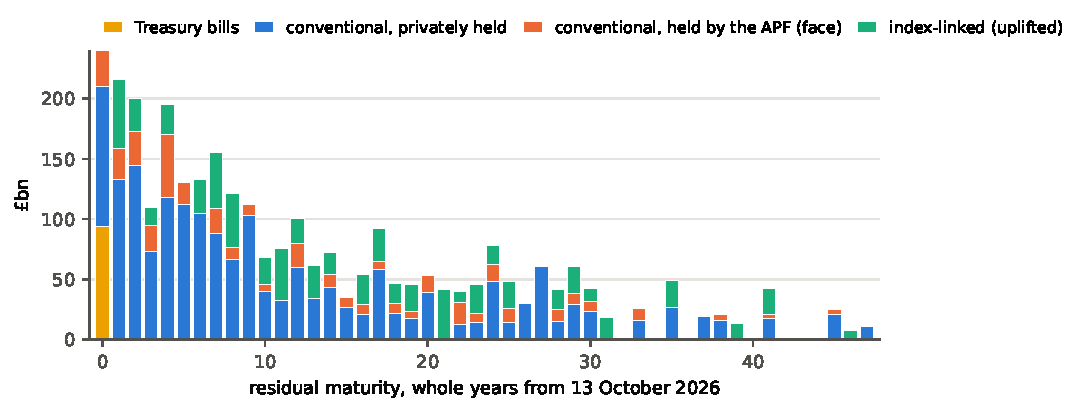
\includegraphics[width=\textwidth]{figures/fig1_uk_profile.pdf}
\caption{UK marketable debt at 12 October 2026 by whole years of residual maturity. APF holdings are shown at face; their historical purchase proceeds total £488.1 billion, not the reported loan balance. The bill profile is reconstructed.}\label{fig:profile}
\end{figure}

\begin{table}[t]\centering\small
\caption{Identified intervals for the increase in UK debt interest, £ billion. Years are 365.25-day model windows from 13 October 2026; bold entries are point-identified. Consolidated panels use the conditional IPP-funded runoff model, not a reconciled OBR perimeter.}\label{tab:uk}
\resizebox{\textwidth}{!}{\begin{tabular}{lrrrr}
\toprule
Disclosure set & Year 1 & Year 3 & Year 5 & Years 1--5 \\
\midrule
\multicolumn{5}{l}{\textit{A. Gross marketable debt, gilt yields +1pp}} \\
Instrument-level value & 0.9 & 4.8 & 7.9 & 22.7 \\
Headline: total, average maturity, IL total, bill stock & 0.0--21.6 & 0.0--22.5 & 0.0--23.5 & 0.0--108.2 \\
DMO brackets: conventional and IL by 0--3, 3--7, 7--15, 15+ years & 0.0--5.6 & 0.0--5.6 & 5.6--11.3 & 11.3--39.5 \\
GFS template: $\le$1, 1--5, $>$5 years; average residual maturity & 0.0--2.4 & 0.0--9.6 & 0.0--9.6 & 0.0--40.8 \\
MTDS cost-risk indicators & 0.0--1.5 & 1.5--22.5 & 1.5--23.4 & 5.8--89.6 \\
Annual profile: amounts and mean dates, years 1--5 & \textbf{0.9} & \textbf{4.8} & \textbf{7.9} & \textbf{22.7} \\
\midrule
\multicolumn{5}{l}{\textit{B. Synthetic IPP-funded, all rates +1pp}} \\
Instrument-level value & 6.4 & 9.8 & 12.3 & 47.7 \\
Headline: total, average maturity, IL total, bill stock & 5.4--27.5 & 5.8--28.4 & 5.8--29.3 & 28.6--137.3 \\
DMO brackets: conventional and IL by 0--3, 3--7, 7--15, 15+ years & 5.4--11.4 & 5.8--11.4 & 7.4--17.1 & 31.8--68.6 \\
GFS template: $\le$1, 1--5, $>$5 years; average residual maturity & 4.9--7.3 & 4.9--14.5 & 4.9--14.5 & 24.4--65.2 \\
MTDS cost-risk indicators & 5.4--7.0 & 7.0--25.2 & 7.0--26.0 & 33.3--106.1 \\
DMO brackets plus APF holdings by bracket & 5.4--10.6 & 5.8--10.6 & 10.6--15.4 & 38.2--62.6 \\
Annual profile: amounts and mean dates, years 1--5 & \textbf{6.4} & \textbf{9.8} & \textbf{12.3} & \textbf{47.7} \\
\midrule
\multicolumn{5}{l}{\textit{C. Synthetic IPP-funded, short rates +1pp}} \\
Instrument-level value & 5.5 & 4.9 & 4.2 & 24.7 \\
Headline: total, average maturity, IL total, bill stock & 0.5--5.8 & 0.9--5.8 & 0.9--5.8 & 4.2--29.1 \\
DMO brackets: conventional and IL by 0--3, 3--7, 7--15, 15+ years & 0.5--5.8 & 0.9--5.8 & 0.9--5.8 & 4.2--29.1 \\
GFS template: $\le$1, 1--5, $>$5 years; average residual maturity & 0.8--7.3 & 0.0--7.3 & 0.0--7.3 & 0.8--36.4 \\
MTDS cost-risk indicators & 4.6--5.8 & 1.4--5.7 & 1.3--5.7 & 10.3--28.5 \\
DMO brackets plus APF holdings by bracket & 4.4--5.8 & 4.9--5.8 & 3.9--4.9 & 22.0--27.3 \\
Annual profile: amounts and mean dates, years 1--5 & \textbf{5.5} & \textbf{4.9} & \textbf{4.2} & \textbf{24.7} \\
\bottomrule
\end{tabular}
}
\end{table}

\paragraph{Headline statistics are nearly uninformative.} With the headline statistics, a one-point rise in gilt yields could add anywhere between nothing and £21.6 billion to first-year interest on the gross portfolio; the gilt-level value is £0.9 billion. Over five years the range is £0--108 billion against £22.7 billion. The width is almost entirely the gap between the convex and concave envelopes in Proposition~\ref{prop:wam}, so it scales with the total and is barely affected by the exact value of average maturity.

\paragraph{Templates help unevenly.} The DMO brackets bound the first three years by the amount in the 0--3-year bracket, but leave the five-year bounds a factor of two or more apart. The international template is narrower for the first year, because its $\le$1-year bucket matches the first window, and wide thereafter, because a 1--5-year bucket says nothing about when within four years debt matures. The MTDS indicators bound the first year well and say almost nothing about later years. Every interval in Table~\ref{tab:uk} reflects a mismatch between bucket edges and the cost windows, as Proposition~\ref{prop:buckets} predicts.

\paragraph{Holdings matter within the declared runoff model.} For the same one-point all-rates shock, the first-year instrument-level model values are £1.65 billion gross and £6.42 billion under the synthetic IPP-funded convention. Historical purchase proceeds of £488 billion enter the latter as a hypothetical funding allocation, not the observed APF loan. Under a short-rate shock (panel C), the headline statistics and DMO brackets give £0.5--5.8 billion against the model value of £5.5 billion. Within this convention, publishing holdings by DMO bracket narrows the five-year short-rate range to £22.0--27.3 billion; annual amounts and mean dates leave only bill-timing uncertainty. These are disclosure effects within a specified model, not evidence that actual APF funding runs off with IPP. Section~\ref{sec:accounting} explains the accounting boundary.

\begin{figure}[t]\centering
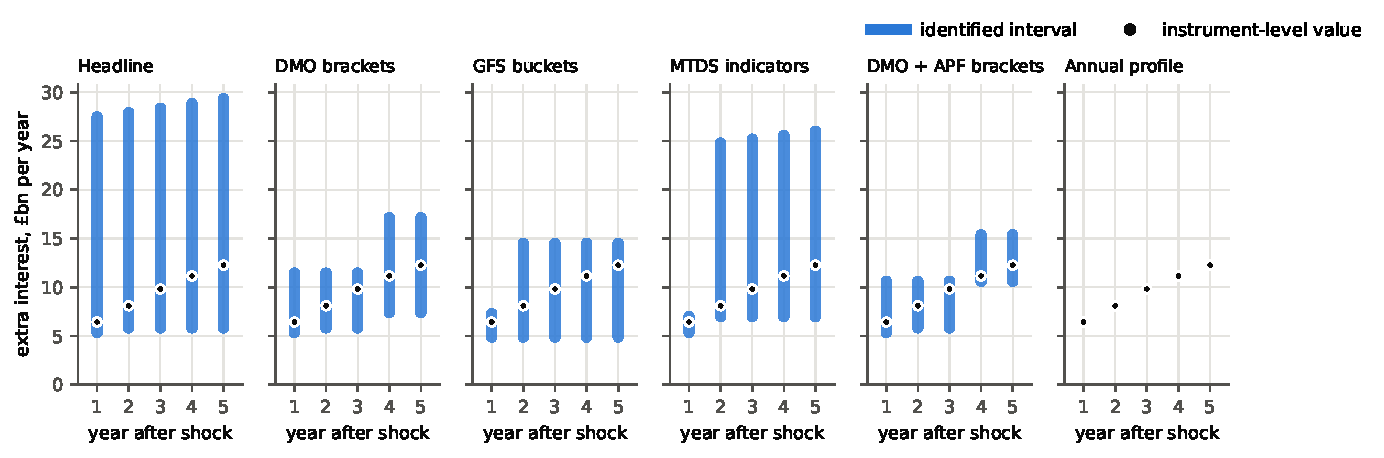
\includegraphics[width=\textwidth]{figures/fig2_uk_consolidated_all.pdf}
\caption{Identified intervals for the synthetic IPP-funded UK exposure to a one-point rise in all rates, by year after the shock, under each disclosure set. Dots mark the instrument-level values.}\label{fig:consall}
\end{figure}

\paragraph{The value of further statistics.} Table~\ref{tab:value} adds candidate statistics to the DMO brackets and reports both the realised and the worst-case width.
\begin{itemize}
\item The share maturing within a year narrows the first-year interval for this portfolio from £6.1 billion to £1.9 billion. Its worst-case width, however, is unchanged at £6.1 billion: had the share been large, the timing of that debt within the year would again have been unknown.
\item The mean maturity of debt due within a year (with the APF part) removes the first-year width entirely, and does so in the worst case.
\item The annual profile of all debt with mean dates is the most valuable statistic for the five-year all-rates exposure, cutting the worst case from £36.8 billion to £20.3 billion. It cannot remove the uncertainty, because the privately held part of the portfolio depends on which gilts the APF holds.
\item For the short-rate exposure no statistic about the gross portfolio helps much. QE holdings by maturity year with mean dates cut the worst-case five-year width from £24.9 billion to £0.5 billion.
\end{itemize}
Against the international template (Table~\ref{tab:value2}), the mean maturity of debt due within a year likewise makes the first-year cost of a common rise in all rates exact, as Corollary~\ref{cor:profile}(iii) predicts. That requires the mean to be published exactly. Table~\ref{tab:precision} shows the price of rounding: a mean rounded to 0.1 years leaves £0.24 billion of width, to 0.01 years £0.024 billion, and to a whole day £0.007 billion. In general the width is at most $\delta$ times the amount due within a year times the rounding interval, because the kernel has slope $-1$ there.

\begin{table}[t]\centering\small
\caption{Width of the identified interval, £ billion, when a specified reporting package is added to the DMO brackets (consolidated perimeter). ``Realised'' uses the statistic's actual value; ``worst case'' is the largest width over all values it could take (Proposition~\ref{prop:coupled}).}\label{tab:value}
\resizebox{\textwidth}{!}{\begin{tabular}{lrrrrrr}
\toprule
Reporting package & \multicolumn{2}{c}{All rates, year 1} & \multicolumn{2}{c}{All rates, years 1--5} & \multicolumn{2}{c}{Short rates, years 1--5} \\
 & realised & worst case & realised & worst case & realised & worst case \\
\midrule
none (base set only) & 6.1 & 6.1 & 36.8 & 36.8 & 24.9 & 24.9 \\
share maturing $<$1y & 1.9 & 6.1 & 32.6 & 35.2 & 23.6 & 24.9 \\
mean maturity of the $<$1y bucket (+ APF part) & 0.0 & 0.0 & 27.2 & 30.7 & 19.6 & 20.0 \\
annual maturity amounts y1-5 & 1.9 & 6.1 & 22.3 & 28.0 & 23.4 & 24.9 \\
mean maturity within DMO brackets & 3.3 & 5.6 & 21.2 & 26.4 & 22.5 & 24.9 \\
annual amounts + mean dates y1-5 & 1.2 & 4.1 & 16.1 & 20.3 & 22.3 & 24.9 \\
APF holdings by DMO bracket & 5.3 & 6.1 & 24.3 & 28.7 & 5.3 & 15.1 \\
APF annual amounts + mean dates y1-5 & 5.3 & 6.1 & 24.7 & 28.7 & 0.5 & 0.5 \\
share refixing $<$1y (consolidated) & 1.6 & 6.1 & 30.0 & 31.2 & 24.9 & 24.9 \\
\bottomrule
\end{tabular}
}
\end{table}

\begin{table}[t]\centering\small
\caption{Width of the identified interval, £ billion, when a specified reporting package is added to the GFS residual-maturity template (gross perimeter).}\label{tab:value2}
\resizebox{0.92\textwidth}{!}{\begin{tabular}{lrrrrrr}
\toprule
Reporting package & \multicolumn{2}{c}{All rates, year 1} & \multicolumn{2}{c}{All rates, years 1--5} & \multicolumn{2}{c}{Gilt yields, year 5} \\
 & realised & worst case & realised & worst case & realised & worst case \\
\midrule
none (base set only) & 2.4 & 2.4 & 31.2 & 31.2 & 9.6 & 9.6 \\
share maturing $<$1y & 2.4 & 2.4 & 31.2 & 31.2 & 9.6 & 9.6 \\
mean maturity of the $<$1y bucket & 0.0 & 0.0 & 28.8 & 28.8 & 9.6 & 9.6 \\
annual maturity amounts y1-5 & 2.4 & 2.4 & 9.6 & 9.6 & 4.3 & 9.6 \\
mean maturity within DMO brackets & 1.5 & 2.4 & 5.2 & 14.4 & 2.7 & 7.2 \\
annual amounts + mean dates y1-5 & 0.0 & 0.0 & 0.0 & 0.0 & 2.4 & 2.4 \\
\bottomrule
\end{tabular}
}
\end{table}

\begin{table}[t]\centering\small
\caption{First-year cost of a one-point rise in all rates, £ billion: the GFS template plus the amount (to £0.1 billion) and mean maturity of debt due within a year, at different publication precisions.}\label{tab:precision}
\resizebox{\textwidth}{!}{\begin{tabular}{lll}
\toprule
Mean maturity of debt due within a year, published & Gross & Synthetic IPP-funded \\
\midrule
exactly & 1.652--1.652 (width 0.000) & 6.424--6.424 (width 0.000) \\
rounded to 0.1 years & 1.557--1.797 (width 0.240) & 6.307--6.576 (width 0.269) \\
rounded to 0.01 years & 1.641--1.665 (width 0.024) & 6.410--6.437 (width 0.027) \\
rounded to one day & 1.651--1.658 (width 0.007) & 6.422--6.430 (width 0.008) \\
Instrument-level value & 1.652 & 6.424 \\
\bottomrule
\end{tabular}
}
\end{table}

\section{The consolidation perimeter}\label{sec:perimeter}

Table~\ref{tab:perimeter} retains alternative mechanical scenarios for comparison. Assigning £99 billion of non-interest-bearing banknotes to the hypothetical funding balance subtracts £0.99 billion per one-point year. This fixed subtraction shifts both endpoints equally and therefore preserves interval widths, but neither that assignment nor the resulting level is a validated whole-Bank consolidation. The sales variant assumes the 2035--2049 block begins running off in April 2027 pro rata. Its extra £0.8 billion reduction in fifth-year short-rate sensitivity is conditional on the stipulated funding retirement, not a measured consequence of the sales notice. Accounting balances, cash flows and their response to the shock must be reconciled before either scenario can be interpreted institutionally.

\begin{table}[t]\centering\small
\caption{Instrument-level values under alternative synthetic funding allocations and runoff scenarios, £ billion. These are imposed scenarios, not validated institutional perimeters.}\label{tab:perimeter}
\resizebox{\textwidth}{!}{\begin{tabular}{llrrrrrr}
\toprule
Perimeter & Shock & Year 1 & Year 2 & Year 3 & Year 4 & Year 5 & Years 1--5 \\
\midrule
Synthetic IPP-funded & all rates & 6.42 & 8.09 & 9.81 & 11.15 & 12.26 & 47.74 \\
Synthetic IPP-funded & short rates & 5.54 & 5.30 & 4.93 & 4.68 & 4.23 & 24.68 \\
Synthetic IPP-funded, with assumed sales & short rates & 5.51 & 5.09 & 4.52 & 4.07 & 3.43 & 22.62 \\
Synthetic banknote allocation & all rates & 5.43 & 7.10 & 8.82 & 10.16 & 11.27 & 42.79 \\
Synthetic banknote allocation & short rates & 4.55 & 4.31 & 3.94 & 3.69 & 3.24 & 19.73 \\
Synthetic banknote allocation, with assumed sales & short rates & 4.52 & 4.10 & 3.53 & 3.08 & 2.44 & 17.67 \\
\bottomrule
\end{tabular}
}
\end{table}

\section{Results for the United States}\label{sec:us}

Table~\ref{tab:us} repeats the exercise for US marketable debt, which is shorter and has more floating-rate debt than the gilt portfolio. With total and average maturity alone, a one-point rise in all rates could add between \$0 and \$275 billion to first-year interest, against a security-level value of \$80 billion; over five years the range is \$0--1,375 billion against \$757 billion. Disclosure by security type pins down the short-rate exposure from the second year, because bills and FRNs then reprice in full, but leaves the bond-yield exposure wide: notes and bonds are defined by original, not residual, maturity, and serve here only as upper bounds on residual maturity. The annual profile by security type identifies the stated annual windows, as in the UK.

\begin{table}[t]\centering\small
\caption{Identified intervals for the increase in US debt interest, \$ billion (gross marketable debt; years from 1 October 2026).}\label{tab:us}
\resizebox{\textwidth}{!}{\begin{tabular}{lrrrr}
\toprule
Disclosure set & Year 1 & Year 3 & Year 5 & Years 1--5 \\
\midrule
\multicolumn{5}{l}{\textit{A. All rates +1pp}} \\
Instrument-level value & 80 & 160 & 205 & 757 \\
Headline: total and average maturity & 0--275 & 0--275 & 0--296 & 0--1375 \\
MSPD summary by security type, average maturity & 7--257 & 78--272 & 78--287 & 320--1286 \\
GFS template: $\le$1, 1--5, $>$5 years; ARM; TIPS total & 0--217 & 106--217 & 106--217 & 426--1085 \\
MTDS cost-risk indicators & 4--110 & 110--271 & 110--284 & 443--1158 \\
Annual profile by security type, years 1--5 & \textbf{80} & \textbf{160} & \textbf{205} & \textbf{757} \\
\midrule
\multicolumn{5}{l}{\textit{B. Short rates +1pp}} \\
Instrument-level value & 65 & 78 & 78 & 378 \\
Headline: total and average maturity & 0--275 & 0--275 & 0--275 & 0--1375 \\
MSPD summary by security type, average maturity & 7--78 & \textbf{78} & \textbf{78} & 320--391 \\
GFS template: $\le$1, 1--5, $>$5 years; ARM; TIPS total & 0--217 & 0--217 & 0--217 & 0--1085 \\
MTDS cost-risk indicators & 4--110 & 4--110 & 4--110 & 18--550 \\
Annual profile by security type, years 1--5 & \textbf{65} & \textbf{78} & \textbf{78} & \textbf{378} \\
\bottomrule
\end{tabular}
}
\end{table}

\section{Robustness and definitional mismatch}\label{sec:robust}

Table~\ref{tab:robust} varies the assumptions behind the bounds. Rounding amounts and maturities to typical published precision moves bucket-based bounds by at most about £0.1 billion. Shares are more fragile: a share rounded to a whole percentage point leaves about £15 billion of debt unplaced, and moves the five-year short-rate lower bound under the MTDS indicators by £1.8 billion. The declared maximum maturity matters only for statistics that involve average maturity: raising it from the longest gilt (47.0 years) to 100 years lifts the headline first-year upper bound from £22.1 billion to £26.5 billion and leaves the bucket-based bounds unchanged. The original first-pass financing approximation at 4.5 per cent raises the synthetic five-year value from £47.7 billion to £52.4 billion. Its bounds are exact for that approximate kernel, not for recursive financing. Section~\ref{sec:recursive} gives a separately specified, exactly recursive annual model and certified results.

Definitional mismatches are a different matter. Each row marked ``mismatch'' computes a statistic under one definition and reads it under another, as a user of published tables might. The actual ledger then violates the statistics as read, so coverage is no longer guaranteed (marked $\ddagger$). In most cases the interval still happens to contain the instrument-level model value. If average maturity weights index-linked gilts at nominal rather than uplifted value, residual maturities are measured from the previous quarter end, or the APF stock at face value is read as purchase cost, the bounds shift but still contain it. If residual-maturity buckets that cover gilts only are read as covering all marketable debt, the bounds exclude the instrument-level model value in three of the nine cases computed: £0.0--1.45 billion for the gross first-year exposure against £1.65 billion, £1.46--8.67 billion in year five against £8.83 billion, and £4.88--6.34 billion for the consolidated first year against £6.42 billion. Nothing in the mis-read statistics themselves signals the error. A prior that is too tight behaves in the same way: restricting QE purchase prices to $[0.9,1.6]$ excludes three actual holdings. Definitions are part of the disclosure.

\begin{table}[t]\centering\small
\caption{Robustness. Identified intervals, £ billion. $\ddagger$: the actual ledger violates a statistic or prior as read, so coverage is not guaranteed; $\dagger$: the interval excludes the instrument-level value. For the first-pass financing approximation row the instrument-level value under that estimand is in parentheses. Dashes mark variants that do not apply.}\label{tab:robust}
\resizebox{\textwidth}{!}{\begin{tabular}{p{.34\textwidth}lll}
\toprule
Variant & \shortstack[l]{Gross\\headline\\year 1} & \shortstack[l]{IPP-funded\\DMO brackets\\years 1--5} & \shortstack[l]{IPP-funded\\GFS template\\year 1} \\
\midrule
Instrument-level value & 1.65 & 47.74 & 6.42 \\
Baseline (exact statistics) & 0.47--22.58 & 31.78--68.57 & 4.88--7.28 \\
Rounded: \pounds0.1bn, 0.1 years, 0.1pp & 0.47--22.58 & 31.77--68.58 & 4.88--7.28 \\
Rounded: \pounds1bn, 0.5 years, 1pp & 0.47--22.58 & 31.70--68.68 & 4.88--7.29 \\
Maximum maturity cap 47.04 years & 0.47--22.09 & 31.78--68.57 & 4.88--7.28 \\
Maximum maturity cap 60 years & 0.47--23.88 & 31.78--68.57 & 4.88--7.28 \\
Maximum maturity cap 100 years & 0.47--26.48 & 31.78--68.57 & 4.88--7.28 \\
Mismatch: WAM weights IL gilts at nominal & 0.47--22.75$^\ddagger$ & 31.78--68.57$^\ddagger$ & 4.88--7.28 \\
Mismatch: maturities measured from 30 Sep & 0.47--22.56$^\ddagger$ & 31.78--68.57$^\ddagger$ & 4.88--7.28$^\ddagger$ \\
Mismatch: GFS buckets exclude T-bills & -- & -- & 4.88--6.34$^{\ddagger\dagger}$ \\
With interest on the extra interest at 4.5\% & 0.48--23.08 (1.69) & 35.10--75.52 (52.44) & 4.99--7.44 (6.57) \\
QE price range $[0.749, 2.354]$ & -- & 31.78--68.57 & 4.88--7.28 \\
QE price range $[0.9, 1.6]$ (excludes three actual holdings) & -- & 31.78--68.57$^\ddagger$ & 4.88--7.28$^\ddagger$ \\
Mismatch: QE stock at face read as purchase cost & -- & 26.21--64.43$^\ddagger$ & 4.05--6.45$^\ddagger$ \\
\bottomrule
\end{tabular}
}
\end{table}

\section{Comparison with the OBR ready reckoner}\label{sec:obr}

The OBR publishes the effect of one-point rises on debt interest net of the APF by fiscal year, starting from the beginning of 2026-27 \citep{OBR2026}. Its figures include new borrowing, NS\&I products, growth in index-linked principal and forecasts of issuance and APF sales; its windows start six months earlier than ours. The proposed reconciliation was not completed. In addition to those differences, the APF funding path used here has not been reconciled to the OBR's accounting convention. Table~\ref{tab:obr} is therefore an unbridged comparison, not external validation. The model's first-year short-rate value is 82 per cent of the OBR entry, but that ratio does not establish common definitions. The frozen-principal inflation illustration is £7.1 billion against the OBR's £7.3 billion. Neither proximity nor divergence identifies the source of the difference without a term-by-term bridge.

\begin{table}[t]\centering\small
\caption{OBR debt-interest ready reckoner (March 2026, fiscal years 2026-27 to 2030-31, read from the published workbook) and the legacy-stock values of this paper (12-month windows from 13 October 2026), £ billion.}\label{tab:obr}
\resizebox{\textwidth}{!}{\begin{tabular}{llrrrrr}
\toprule
 & & 1 & 2 & 3 & 4 & 5 \\
\midrule
Short rates +1pp & OBR, fiscal years 2026-27 to 2030-31 & 6.73 & 6.91 & 6.32 & 5.81 & 5.04 \\
 & Synthetic IPP-funded & 5.54 & 5.30 & 4.93 & 4.68 & 4.23 \\
 & Synthetic IPP-funded, with assumed sales & 5.51 & 5.09 & 4.52 & 4.07 & 3.43 \\
 & Synthetic banknote allocation & 4.55 & 4.31 & 3.94 & 3.69 & 3.24 \\
 & Synthetic banknote allocation, with assumed sales & 4.52 & 4.10 & 3.53 & 3.08 & 2.44 \\
Gilt yields +1pp & OBR, fiscal years 2026-27 to 2030-31 & 1.23 & 3.71 & 6.24 & 8.39 & 10.36 \\
 & Synthetic IPP-funded & 0.88 & 2.79 & 4.88 & 6.47 & 8.03 \\
RPI inflation +1pp & OBR, fiscal years 2026-27 to 2030-31 & 7.33 & 8.48 & 9.18 & 9.60 & 10.51 \\
 & Synthetic IPP-funded & 5.19 & 7.12 & 7.12 & 7.12 & 7.12 \\
\bottomrule
\end{tabular}
}
\end{table}

\section{Accounting reconciliation and its information boundary}\label{sec:accounting}

The Bank's weekly report and operational stock page both refer to 7 October 2026 \citep{BoEweekly,BoEusage}. They report an APF loan of \pounds521,819 million and gilt holdings of \pounds488,149 million at initial purchase proceeds, respectively. The latter is a historical purchase-cost measure after removing the IPP of sold or redeemed holdings, not their sale proceeds or the current loan. The manuscript's more precise workbook sum is \pounds488,149.275 million. Subtracting it from the rounded loan gives \pounds33,669.725 million, but this is neither measured net funding nor an established correction to the results.

A dated observation from 7 October is usable on 13 October. The limitation is not that October is unfinished: it is the absence of matched cash/principal information and future cash-flow paths. The annual accounts at 28 February 2026 \citep{BoEaccounts} provide a different-date check, in \pounds million:
\[
21{,}714+382{,}080+150{,}677+51=554{,}522.
\]
The terms are cash, securities at fair value, indemnity asset and other assets; the right side is the loan liability. Notes 6--7 state that cash earns Bank Rate and that the loan includes principal and accrued interest. February balances cannot be inserted into October calculations. These observations follow the Bank's accounts and weekly/operational records, not a new accounting theory.

More generally let $V,C,I,A,L,O,E$ denote securities carrying value, cash, indemnity receivable, other assets, loan liability, other liabilities and equity. Then
\[
L-P=(V-P)+C+I+A-O-E,
\]
where $P$ is remaining IPP. For loan principal $L_p$, purchases $X$, cash proceeds $R$, coupons $K$, cash-deposit interest $I_C$, loan interest $I_L$, costs $F$ and indemnity cash receipts $T$ from the Treasury, cash conservation gives
\begin{align*}
\Delta C&=\Delta L_p-X+R+K+I_C-I_L-F+T,\\
\Delta(L_p-P)&=\Delta C+(D-R)-K-I_C+I_L+F-T,
\end{align*}
where $D$ is the IPP removed and $\Delta P=X-D$. Loan carrying values additionally require accrued-interest changes. The available October sources do not identify all these terms or their future paths. Under fixed balances and equal repricing, direct net financing sensitivity involves $L_p-C$, not $L$ or $P$. Whole-Bank consolidation instead cancels internal loans and deposits and requires external reserves and offsetting assets. A fixed banknote subtraction cannot establish that perimeter.

Accordingly all legacy \texttt{consolidated} and \texttt{consolidated\_bank} results are retained as explicitly synthetic allocation/runoff scenarios. Their certificates establish model optima, not observed consolidated fiscal exposure. The unsupported institutional equivalence is withdrawn. No numerical residual accounting bound is claimed from these sources.

\begin{proposition}[Conditional accounting-error envelope]\label{prop:accounting}
Suppose a declared experiment has $J_{\rm target}=J_{\rm proxy}+\int_a^b s(t)q(t)\,dt$, with known shock $s$ and externally justified pointwise bounds $q_-\le q\le q_+$. Assume these functions are measurable and the products $sq,sq_-,sq_+$ are integrable. If $L\le J_{\rm proxy}\le U$, then the target lies between
\[
L+\int_a^b\min\{sq_-,sq_+\}\,dt
\quad\hbox{and}\quad
U+\int_a^b\max\{sq_-,sq_+\}\,dt.
\]
These bounds are sharp if $L,U$ are attained sharp proxy endpoints, the portfolio and residual feasible sets form a Cartesian product, and the sign-selected paths attaining the displayed residual extrema are feasible. Otherwise they are only enclosing bounds.
\end{proposition}
\begin{proof}
Multiply the pointwise bounds by the signed shock, take the smaller and larger products and integrate. Add the proxy bounds. Under the product assumption each proxy extremum can be combined with the corresponding extremal residual path; without it this combination need not be feasible.
\end{proof}
Here $q$ is net repricing principal omitted by the proxy; other accounting differences must either be fixed or included explicitly in the error model. Even knowing $q(0)$ does not control its multi-year integral. A hypothetically constant extra \pounds33.669725 billion would contribute \pounds0.33669725 billion per one-percentage-point year, but neither constancy nor that net amount is established. This example is a sensitivity calculation, not a corrected estimate or confidence interval.

\subsection{A source-backed historical accounting check}
The February 2026 annual accounts allow a reconciliation that the October holdings snapshot does not. All amounts below are in \pounds million, as reported, not inferred from gilt purchase cost. The cash-flow statement gives
\[
13{,}304+134{,}833-101{,}372-25{,}051=21{,}714.
\]
Opening cash, net operating cash, loan repayments and interest paid thus reproduce closing cash exactly at the published precision. The carrying-value roll-forward is
\[
656{,}387-101{,}372+24{,}559-25{,}051=554{,}523,
\]
within \pounds1 million of the reported \pounds554,522 million closing loan, consistent with independently rounded statement lines. Accrued interest therefore matters even for the historical stock reconciliation. These are reproductions of the accounts, not new empirical discoveries.

For a narrowly defined sensitivity, hold the February principal and cash deposit fixed, let both reprice equally, and exclude all valuation, issuance, indemnity and behavioural responses. A permanent one-percentage-point change then changes the APF's direct annualised net financing charge by $0.01(L_p-C)$. The accounts report $L_p=\pounds553.2$ billion to one decimal place and $C=\pounds21{,}714$ million to the nearest million. Under conventional nearest-unit rounding their implied interval is
\[
0.01(L_p-C)\in[\pounds5.314355,\pounds5.315365]\ \text{billion per year}.
\]
This is an interval due to publication precision for a frozen-balance derivative, not a confidence interval, a forecast, the full public-sector net interest cost, or an October estimate. It demonstrates how a correctly defined accounting target can enter the bounding framework. Extending it over five years requires a cash/funding path and its shock response; the annual statements do not supply that path.

\paragraph{Independent source retrieval for the gilt ledger.} On 13 October an ordinary browser download from the official DMO report succeeded. Its internal heading is ``Gilts in issue on 12 October 2026''. All 105 ISINs, instrument types, redemption dates, nominal amounts and inflation-uplifted amounts agree with the supplied XML; the largest amount discrepancy is $10^{-11}$ million pounds, attributable to spreadsheet floating-point representation. The archived spreadsheet and row-by-row checker remove the earlier authentication gap for these computationally relevant gilt fields. This does not turn reconstructed bill timing into observed data or establish the APF funding model. The comparison is producer-coordinated source verification, not unaffiliated reproduction.


\section{Exactly recursive annual financing}\label{sec:recursive}
The original \texttt{iai} kernel is an annual-midpoint \emph{first-pass approximation}: it pays interest on previous first-round costs, not on accumulated financing interest. Exact optimisation of that kernel does not make it exact continuous-time financing.

An alternative declared discrete convention books each year's first-round cost $C_k$ at the midpoint, charges it half-year simple interest at rational rate $y\ge0$, and charges the prior accumulated extra debt a full year of simple interest. With $B_0=0$,
\[
B_k=(1+y)B_{k-1}+(1+y/2)C_k,\qquad
B_H=(1+y/2)\sum_{j=1}^H(1+y)^{H-j}C_j.
\]
This is exact for that convention by induction. Year-$k$ cost is $B_k-B_{k-1}$. Each $C_j$ is a piecewise-affine linear functional of the ledger, so the same is true of these rational weighted sums and the existing reduction and certificates apply. At $y=0.045$, the synthetic IPP-funded five-year value is \pounds52.678453 billion, versus \pounds52.443165 billion for first-pass financing and \pounds47.735924 billion without it. We supply 36 additional exact endpoint certificates for this convention. None validates the APF accounting.

Continuous recursive financing instead weights a constant flow beginning at $\tau$ by $(e^{y(H-\tau)^+}-1)/y$. It remains linear in amounts but not piecewise affine in maturity. We do not apply the breakpoint lemma to it or claim the annual convention equals it. The review's approximately \pounds52.753124 billion continuous calculation is a useful convention comparison, not a separately certified result of this release.


\section{Related work}\label{sec:lit}

Practitioner guidance already warns that average maturity can hide concentrated redemptions and recommends looking at redemption profiles \citep{IMFWB2014,JonassonPapaioannou2018}. \citet{BarrettJohns2024} fit parametric maturity structures to full payment schedules for six countries. Neither computes the set of cost outcomes consistent with the indicators. In banking, the Basel standardised measure of interest-rate risk in the banking book assumes that cash flows within a time band match perfectly, and relies on the number of bands to mitigate the error \citep{BCBS2019}; \citet{EntropWilkensZeisler2009} show that the measure is sensitive to such assumptions but do not compute sharp bounds. Immunisation theory bounds the interest-rate exposure of a portfolio from moments of its cash-flow timing, notably the dispersion bound of \citet{FongVasicek1984} building on \citet{Redington1952}; it bounds value changes under non-parallel shifts for a known portfolio rather than cost outcomes over all portfolios consistent with a disclosure. On consolidation, the OBR \citep{OBR2021box} and US Treasury's consolidated next-rate-reset measures \citep{TBAC2026} compute point values from security-level holdings. The euro area offers a live case of aggregate-only disclosure: holdings under the public-sector purchase programme are published only as book value and weighted average residual maturity by issuer country \citep{ECB2020}.

The mathematics is classical. Bounds on expectations given moments go back to \citet{Rogosinski1958} and \citet{Kemperman1968}, with finite-support extremals as in \citet{Winkler1988}. The bucket results are the Jensen and Edmundson--Madansky bounds and their partition refinements \citep{Madansky1959,HuangZiembaBenTal1977,BirgeWets1986}. Bounds on expected payoffs of the form $(h-t)^+$ appear in actuarial stop-loss theory \citep{DeVylderGoovaerts1982,JansenHaezendonckGoovaerts1986} and in option pricing \citep{Lo1987,BertsimasPopescu2002,BertsimasPopescu2005}. Sharp bounds by linear programming are standard in partial identification \citep{ManskiTamer2002,MogstadSantosTorgovitsky2018}, and \citet{Gastwirth1972} bounded the Gini index from grouped data. Exact verification of linear programmes follows \citet{ApplegateEtAl2007} and \citet{GleixnerSteffyWolter2016}. The application to published debt statistics, the set identification of consolidated exposure when central-bank holdings are disclosed only in aggregate, and the worst-case value of additional statistics were not found in the searches made for this study (literature databases, debt-office and central-bank publications, to 13 October 2026). Some sources were inaccessible, and the searches are not exhaustive.

\section{Implications for disclosure}\label{sec:implications}

The results support four practical recommendations.
\begin{enumerate}
\item Publish, for each rate leg, the amounts and mean refixing dates of debt refixing in each of the next five years, with the amount refixing later and, for index-linked debt, the split by indexation lag. These identify the first-order cost of every permanent shock in every year of the horizon, and of every year-by-year path for fixed-rate debt and continuously resetting floating debt. For bills under paths that change between years, tenors and rollover dates are also needed.
\item Where a central bank holds government debt, publish maturity-resolved holdings with valuation definitions, but also reconcile loan principal, accrued interest, cash, indemnity flows and the assumed future funding path. Holdings alone do not identify actual consolidated sensitivity. Do not assign banknotes to a particular asset portfolio without an explicit consolidation model.
\item In the international residual-maturity template, add the mean maturity of the $\le$1-year bucket, published to the day. One number then pins the first-year cost of a common rise in rates to within £0.01 billion for the UK.
\item State definitions with the numbers: which instruments a bucket covers, whether index-linked debt is weighted at nominal or uplifted value, and whether central-bank holdings are at face or at purchase cost. A wrong reading can produce confident bounds that exclude the instrument-level model value, with nothing in the statistics to reveal it.
\end{enumerate}
A ready reckoner such as the OBR's remains the most direct statement of sensitivity for its own scenarios. The annual profile complements it by letting any user compute the sensitivity to permanent shocks in the stated annual windows.

\paragraph{Limitations.} The estimand is first-order and accounting-based. It holds amounts fixed, refinances like-for-like, keeps index-linked principal frozen, and ignores behavioural responses and the effect of the shock on deficits. It is not a probability of any outcome. The synthetic funding level depends on the declared allocation (Section~\ref{sec:perimeter}). The UK bill profile is reconstructed; computationally relevant fields of the re-entered gilt list have now been checked against the official dated spreadsheet. The bounds are sharp only for the stated model of the ledger. If the model omits a liability or misassigns a rate leg, the bounds can exclude the instrument-level model value, exactly as a definitional mismatch can.

\section*{Reproducibility and method statement}
The accompanying code produces the original results tables, including the OBR comparison, from the sources listed in Section~\ref{sec:data}; their provenance and SHA-256 hashes are retained. Restricted BoE and OBR originals are not redistributed. Source-based regeneration requires the matching historical inputs; current URLs may change vintage. The public archive also supplies exact model snapshots: all 4,540 original and 36 additional recursive-annual certificates can be checked offline against those models and linked exactly to the reported values, using only Python's standard library. The producer separately checked equality between snapshots and the source-based builder. A second evaluator, with its own parsers for the raw files, recomputes original instrument-level values and agrees to $10^{-9}$; it shares the modelling conventions, so it checks implementation, not assumptions. The test suite checks the bounds against the closed forms of Section~\ref{sec:theory} on random portfolios, annual-profile exactness, grid refinement, daily-grid attainment, rounded statistics and data integrity. Negative controls must reject altered certificate values, missing witnesses, incorrect senses and malformed dual rows even with assertions disabled. AI systems assisted the analysis, programming, drafting and adversarial checking; this is not human peer review or unaffiliated reproduction. The evidence rests on the stated arguments, certificates and tests, not model agreement.

\begin{thebibliography}{99}\small
\bibitem[Bank of England(2026c)]{BoEweekly} Bank of England (2026c). Weekly report, 7 October 2026. \url{https://www.bankofengland.co.uk/weekly-report/2026/7-october-2026}.
\bibitem[Bank of England(2026d)]{BoEusage} Bank of England (2026d). Market operations guide: results and usage data, APF stock as at 7 October 2026. \url{https://www.bankofengland.co.uk/markets/bank-of-england-market-operations-guide/results-and-usage-data}. Accessed 13 October 2026.
\bibitem[Bank of England(2026e)]{BoEaccounts} Bank of England Asset Purchase Facility Fund Limited (2026e). Annual report and accounts 2025/26, statement of financial position and notes 6--7, 10 and 14. \url{https://www.bankofengland.co.uk/-/media/boe/files/asset-purchase-facility/2026/apf-annual-report-2025-26.pdf}.
\bibitem[Applegate et~al.(2007)]{ApplegateEtAl2007} Applegate, D.~L., Cook, W., Dash, S. and Espinoza, D.~G. (2007). Exact solutions to linear programming problems. \emph{Operations Research Letters} 35(6), 693--699.
\bibitem[Bank of England(2026a)]{BoE2026notice} Bank of England (2026a). Asset Purchase Facility gilt sales: market notice, 17 September 2026.
\bibitem[Bank of England(2026b)]{BoE2026notes} Bank of England (2026b). The promise to pay: what backs banknotes? Bank Insights, September 2026.
\bibitem[Barrett and Johns(2024)]{BarrettJohns2024} Barrett, P. and Johns, C. (2024). Parameterizing debt maturity. \emph{Journal of Money, Credit and Banking} 56(6), 1321--1365. doi:10.1111/jmcb.13116. Accessible precursor: IMF Working Paper 2021/101.
\bibitem[BCBS(2019)]{BCBS2019} Basel Committee on Banking Supervision (2019). SRP31: Interest rate risk in the banking book. Basel Framework.
\bibitem[Bertsimas and Popescu(2002)]{BertsimasPopescu2002} Bertsimas, D. and Popescu, I. (2002). On the relation between option and stock prices: a convex optimization approach. \emph{Operations Research} 50(2), 358--374.
\bibitem[Bertsimas and Popescu(2005)]{BertsimasPopescu2005} Bertsimas, D. and Popescu, I. (2005). Optimal inequalities in probability theory: a convex optimization approach. \emph{SIAM Journal on Optimization} 15(3), 780--804.
\bibitem[Birge and Wets(1986)]{BirgeWets1986} Birge, J.~R. and Wets, R.~J.-B. (1986). Designing approximation schemes for stochastic optimization problems, in particular for stochastic programs with recourse. \emph{Mathematical Programming Study} 27, 54--102.
\bibitem[De Vylder and Goovaerts(1982)]{DeVylderGoovaerts1982} De Vylder, F. and Goovaerts, M. (1982). Analytical best upper bounds on stop-loss premiums. \emph{Insurance: Mathematics and Economics} 1(3), 163--175.
\bibitem[ECB(2020)]{ECB2020} European Central Bank (2020). Decision (EU) 2020/188 on a secondary markets public sector asset purchase programme (ECB/2020/9).
\bibitem[Entrop et~al.(2009)]{EntropWilkensZeisler2009} Entrop, O., Wilkens, M. and Zeisler, A. (2009). Quantifying the interest rate risk of banks: assumptions do matter. \emph{European Financial Management} 15(5), 1001--1018.
\bibitem[Fong and Vasicek(1984)]{FongVasicek1984} Fong, H.~G. and Vasicek, O.~A. (1984). A risk minimizing strategy for portfolio immunization. \emph{Journal of Finance} 39(5), 1541--1546.
\bibitem[Gastwirth(1972)]{Gastwirth1972} Gastwirth, J.~L. (1972). The estimation of the Lorenz curve and Gini index. \emph{Review of Economics and Statistics} 54(3), 306--316.
\bibitem[Gleixner et~al.(2016)]{GleixnerSteffyWolter2016} Gleixner, A.~M., Steffy, D.~E. and Wolter, K. (2016). Iterative refinement for linear programming. \emph{INFORMS Journal on Computing} 28(3), 449--464.
\bibitem[Huang et~al.(1977)]{HuangZiembaBenTal1977} Huang, C.~C., Ziemba, W.~T. and Ben-Tal, A. (1977). Bounds on the expectation of a convex function of a random variable: with applications to stochastic programming. \emph{Operations Research} 25(2), 315--325.
\bibitem[IMF and World Bank(2014)]{IMFWB2014} International Monetary Fund and World Bank (2014). Revised guidelines for public debt management. IMF Policy Paper.
\bibitem[IMF and World Bank(2019)]{IMFWB2019} International Monetary Fund and World Bank (2019). Developing a medium-term debt management strategy (MTDS): updated guidance note for country authorities.
\bibitem[Jansen et~al.(1986)]{JansenHaezendonckGoovaerts1986} Jansen, K., Haezendonck, J. and Goovaerts, M.~J. (1986). Upper bounds on stop-loss premiums in case of known moments up to the fourth order. \emph{Insurance: Mathematics and Economics} 5(4), 315--334.
\bibitem[Jonasson and Papaioannou(2018)]{JonassonPapaioannou2018} Jonasson, T. and Papaioannou, M.~G. (2018). A primer on managing sovereign debt-portfolio risks. IMF Working Paper 18/74.
\bibitem[Kemperman(1968)]{Kemperman1968} Kemperman, J.~H.~B. (1968). The general moment problem, a geometric approach. \emph{Annals of Mathematical Statistics} 39(1), 93--122.
\bibitem[Lo(1987)]{Lo1987} Lo, A.~W. (1987). Semi-parametric upper bounds for option prices and expected payoffs. \emph{Journal of Financial Economics} 19(2), 373--387.
\bibitem[Madansky(1959)]{Madansky1959} Madansky, A. (1959). Bounds on the expectation of a convex function of a multivariate random variable. \emph{Annals of Mathematical Statistics} 30(3), 743--746.
\bibitem[Manski and Tamer(2002)]{ManskiTamer2002} Manski, C.~F. and Tamer, E. (2002). Inference on regressions with interval data on a regressor or outcome. \emph{Econometrica} 70(2), 519--546.
\bibitem[Mogstad et~al.(2018)]{MogstadSantosTorgovitsky2018} Mogstad, M., Santos, A. and Torgovitsky, A. (2018). Using instrumental variables for inference about policy relevant treatment parameters. \emph{Econometrica} 86(5), 1589--1619.
\bibitem[OBR(2021)]{OBR2021box} Office for Budget Responsibility (2021). Debt maturity, quantitative easing and interest rate sensitivity. Box in \emph{Economic and fiscal outlook}, March 2021.
\bibitem[OBR(2026)]{OBR2026} Office for Budget Responsibility (2026). \emph{Economic and fiscal outlook}, March 2026: detailed forecast tables, debt interest ready reckoner.
\bibitem[Redington(1952)]{Redington1952} Redington, F.~M. (1952). Review of the principles of life-office valuations. \emph{Journal of the Institute of Actuaries} 78(3), 286--340.
\bibitem[Rogosinski(1958)]{Rogosinski1958} Rogosinski, W.~W. (1958). Moments of non-negative mass. \emph{Proceedings of the Royal Society of London A} 245(1240), 1--27.
\bibitem[TBAC(2026)]{TBAC2026} Treasury Borrowing Advisory Committee (2026). Bill purchases and the consolidated balance sheet. Charge presentation, 3 February 2026.
\bibitem[Winkler(1988)]{Winkler1988} Winkler, G. (1988). Extreme points of moment sets. \emph{Mathematics of Operations Research} 13(4), 581--587.
\end{thebibliography}

\appendix
\section{Further figures}
\begin{figure}[h]\centering
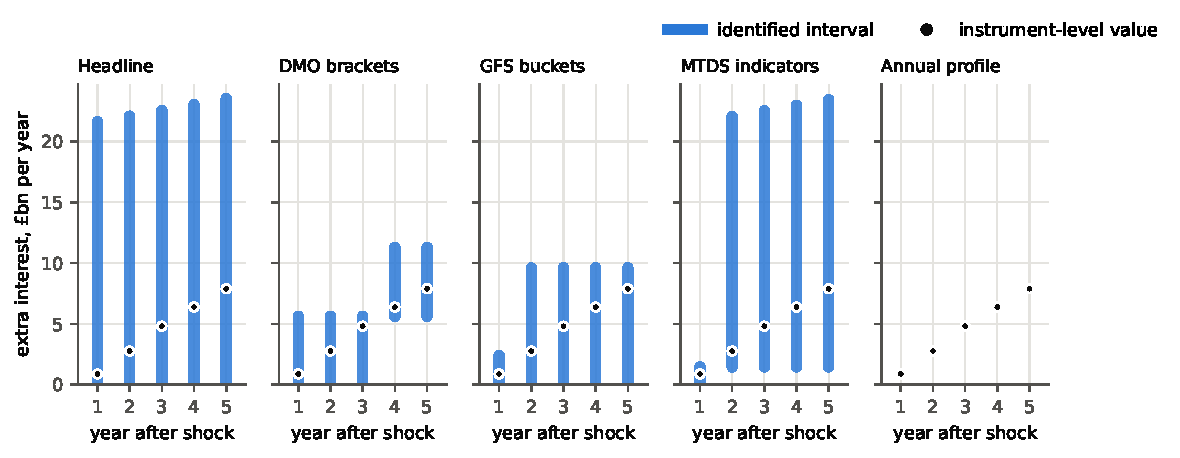
\includegraphics[width=0.95\textwidth]{figures/fig3_uk_gross_gilt.pdf}
\caption{Identified intervals for the gross UK exposure to a one-point rise in gilt yields.}
\end{figure}
\begin{figure}[h]\centering
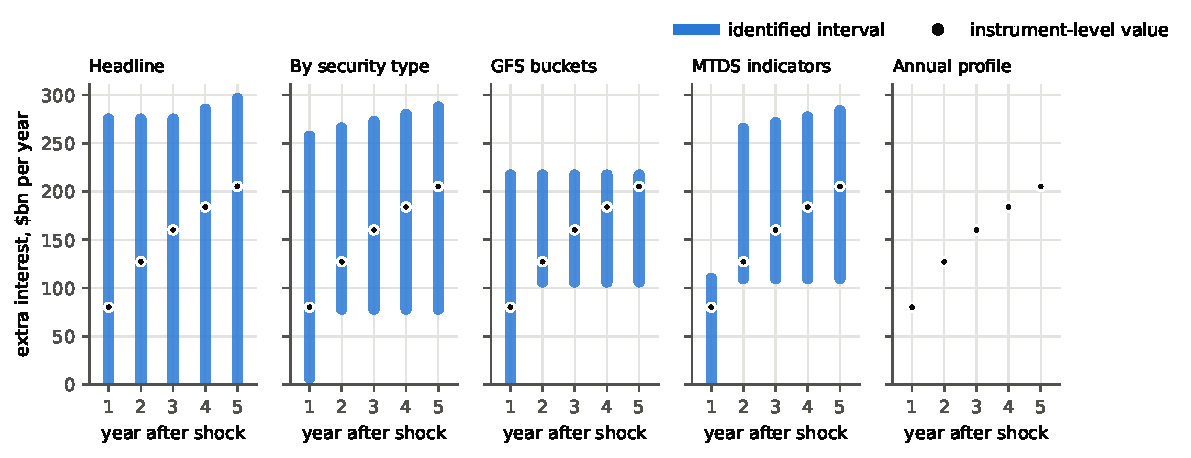
\includegraphics[width=0.95\textwidth]{figures/fig5_us_all.pdf}
\caption{Identified intervals for the US exposure to a one-point rise in all rates.}
\end{figure}
\begin{figure}[h]\centering
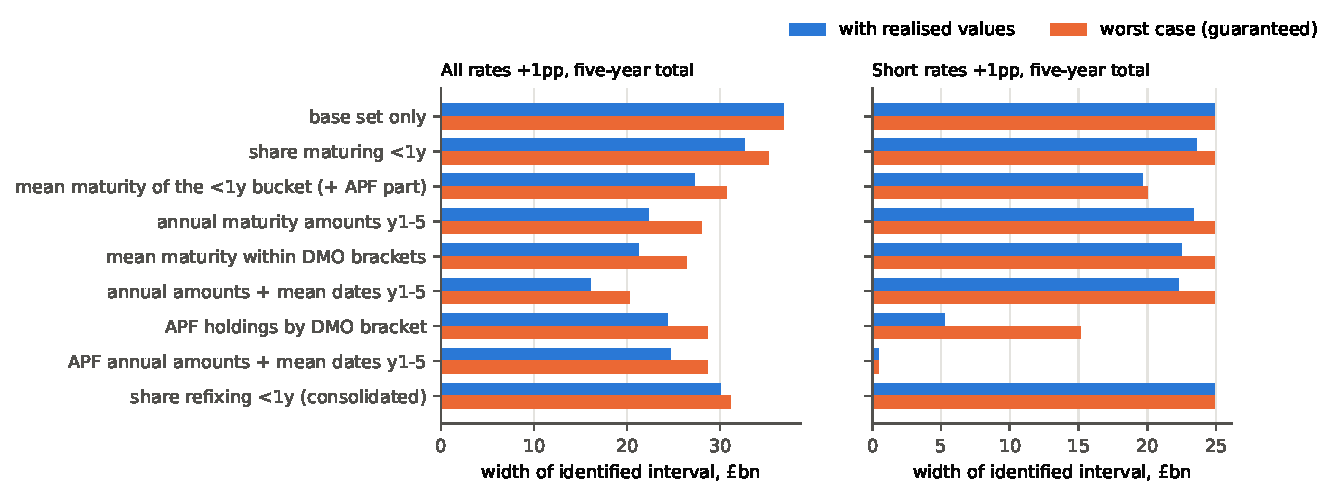
\includegraphics[width=\textwidth]{figures/fig4_uk_value_of_disclosure.pdf}
\caption{Realised and worst-case widths when a specified reporting package is added to the DMO brackets (consolidated perimeter), five-year totals.}
\end{figure}

\end{document}
